\documentclass[a4paper]{article}
\usepackage[utf8]{inputenc}
\usepackage[a4paper, left=2.5cm, right=2.5cm, top=2cm, bottom=2cm]{geometry}
\usepackage{lmodern}
\usepackage[T1]{fontenc}
\usepackage{graphicx}
\usepackage{amssymb}
\usepackage[utf8]{inputenc}
\usepackage{pgfplots}
\pgfplotsset{width=6cm,compat=1.9}
\usepackage{multicol}
\usepackage{csquotes}

\renewcommand{\thesection}{\Alph{section}}
\renewcommand{\thesubsection}{\arabic{subsection}}
\renewcommand{\thesubsubsection}{(\emph{\alph{subsubsection}})}

\title{Logarithme}
\author{Hugo Lageneste}
\date{Janvier 2020}

\begin{document}

{Mathématiques - Logarithme}

\begin{center}
 \newcommand{\HRule}{\rule{\linewidth}{0.5mm}}
 {\huge \bfseries Logarithme}\\[0.1cm]
\end{center}

\section{Propriétés du logarithme népérien}
\subsection{Caractérisation}

{La fonction logarithme népérien notée $\ln{}$ et définie sur $I=\mathbb{R}^{+*}$ est définie par:}

\[\ln{x}=y \Leftrightarrow x=e^y\]

{Le logarithme népérien est donc le réciproque de l'exponentielle}

\[\forall x \in \mathbb{R}^{+*}, \ln{e^x}=x\]
\[\forall x \in \mathbb{R}^{+*}, e^{\ln{x}}=x\]

\subsection{Signe}

\begin{multicols}{2}
	\begin{itemize}
  		\item{$\forall x \in ]0;1]$, $\ln{x} \leqslant 0$}
  		\item{$\forall x \in [1;+\infty[$, $\ln{x} \geqslant 0$}
	\end{itemize}
\end{multicols}

\begin{center}
	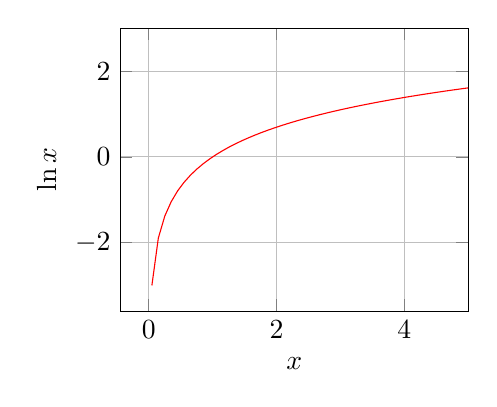
\begin{tikzpicture}
		\begin{axis}[grid=major,  xmax=5, ymax=3, samples=100, xlabel=$x$, ylabel=$\ln{x}$]
			\addplot[color=red]{ln(x)};
		\end{axis}
	\end{tikzpicture}
\end{center}

\subsection{Propriétés}

{$\forall x \in \mathbb{R}^{+*}$:}

\begin{multicols}{3}
	\begin{itemize}
  		\item{$\ln{xy}=\ln{x}+\ln{y}$}
  		\item{$\ln{\frac{x}{y}=\ln{x}-\ln{y}}$}
  		\item{$\ln{\frac{1}{x}}=-\ln{x}$}
	\end{itemize}
\end{multicols}
{$\forall x \in \mathbb{R}^{+*}$ et $\forall n \in \mathbb{Z}$:}

\begin{multicols}{2}
	\begin{itemize}
		\item{$\ln{x^n}=n\ln{x}$}
		\item{$\ln{\sqrt{x}}=\frac{1}{2}\ln{x}$}
	\end{itemize}
\end{multicols}

\section{Étude du logarithme népérien}
\subsection{Limites}
\subsubsection{Limites}

{Aux bornes de son ensemble de définition, les limites du logarithme népérien sont:}

\begin{multicols}{2}
	\begin{itemize}
  		\item{$\lim\limits_{x \rightarrow 0^+} \ln{x}=-\infty$}
  		\item{$\lim\limits_{x \rightarrow +\infty} \ln{x}=+\infty$}
	\end{itemize}
\end{multicols}

\subsubsection{Croissances comparées}

\begin{multicols}{2}
	\begin{itemize}
  		\item{$\lim\limits_{x \rightarrow +\infty} \frac{\ln{x}}{x}=0$}
  		\item{$\lim\limits_{x \rightarrow 0^+} x\ln{x}=0$}
	\end{itemize}
\end{multicols}

\subsection{Dérivée}
\subsubsection{Dérivée de $\ln{x}$}

{$\ln{x}$ est dérivable sur $\mathbb{R}^{+*}$ et}

\[\ln{}\prime x = \frac{1}{x}\]

\subsubsection{Dérivée de $\ln{u}$}

{$u$ est une fonction dérivable et strictement positive sur $I$, $\ln{u}$ est alors dérivable sur $I$}

\[\forall x \in I, \left(\ln{u}\right)\prime(x)=\frac{u\prime(x)}{u(x)}\]

\subsection{Logarithme décimal}
\subsubsection{Définition}

{La fonction logarithme décimal est définie sur $\mathbb{R}^{+*}$ est définie par}

\[\log{x}=\frac{\ln{x}}{\ln{10}}\]

\subsubsection{Propriétés}

{$\forall n \in \mathbb{N}$:}

\begin{multicols}{2}
	\begin{itemize}
  		\item{$\log{10}=1$}
  		\item{$\log{10^n}=n$}
	\end{itemize}
\end{multicols}

\end{document}